\def\difficulty{1}
\sujet{Multiscale Analysis}
\label{lbl:tutorial:multiscale}
\index{Multiscale}

\begin{note}This tutorial aims to study some multiscale image processing and analysis methods, based on pyramidal and scale-space representations.\end{note}

\noindent The different processes will be applied on the following MR image.
\begin{figure}[h]
\begin{center}
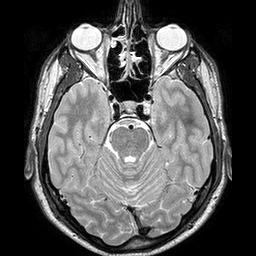
\includegraphics[width=3.25cm]{cerveau.jpg}
\caption{Brain MR image.}
\end{center}
\vspace*{-8pt}
\end{figure}

\vspace*{-12pt}

\section{Pyramidal decomposition and re\-cons\-truc\-tion}
\index{Multiscale!Pyramid}

\vspace*{-4pt}
\subsection{Decomposition}


\begin{algorithm}[H]
\SetAlgoLined
\KwData{image $A_0$}
\KwResult{pyramid of approximations $\{A_i\}_i$, pyramid of details$\{D_i\}_i$}
\For{i=1 to 3}{
	filtering: $F=filt(A_{i-1})$\;
	 subsampling: $A_i=ech(F,0.5)$\;
	 details: $D_i=A_{i-1}-ech(A_i,2)$\;
}
\caption{The algorithm of the pyramidal decomposition}
\end{algorithm}

The initial image (with the highest resolution), denoted $A_0$, represents the level 0 of the pyramid.
To build the pyramid, we successively carry out the following steps:
\begin{enumerate}
	\item a Gaussian filtering,
	\item a subsampling,
	\item a calculation of the details (residues).
\end{enumerate}

\begin{qbox}Make a pyramidal decomposition with 4 levels of the image 'brain'.
\end{qbox}


\begin{mcomment}
\begin{mremark}
You can use the \matlabregistered{} command \minline{cell} to store the images of the different levels of the pyramid. \minline{imfilter} and \minline{fspecial} will be used to perform the filtering process, \minline{imresize} is used to down- or over-sampling the image.
\end{mremark}
\end{mcomment}

\vspace*{-4pt}
\subsection{Reconstruction} 
To reconstruct the original image, we carry out the following steps at each level of the pyramid:
\begin{enumerate}
	\item an oversampling,
	\item an addition of the details.
\end{enumerate}

\newpage

%\noindent The algorithm of the pyramidal reconstruction is given below:

\begin{algorithm}[H]
\SetAlgoLined
\KwData{image $A_3$, pyramid of details$\{D_i\}_i$}
\KwResult{reconstructed pyramid $\{B_i\}_i$}
initialization : $B_3=A_3$\;
\For{i=3 to 1}{
 \nl oversampling: $R=ech(B_i,2)$\;
	\nl adding details: $B_{i-1}=R+D_i$
}
\caption{The algorithm of the pyramidal reconstruction}
\end{algorithm}

\begin{qbox}
\begin{enumerate}
	\item Reconstruct the original image from the last level of the pyramid.
	\item Make the same reconstruction without adding the details.
	\item Calculate the resulting error between the reconstruted image and the original image.
\end{enumerate}
\end{qbox}

\section{Scale-space decomposition and mul\-ti\-scale fil\-te\-ring}
\index{Multiscale!Filtering}

\textls[-25]{We are going to decompose (without any sampling) the image with the highest resolution with a morphological operator, dilation or erosion. The resulting images will have the same size.}

\subsection{Morphological multiscale  decomposition}
\begin{qbox}
Build the two scale-space decompositions of the 'brain' image, with a disk of increasing radius as a structuring element
\end{qbox}

\begin{mcomment}
\begin{mremark}See the \matlabregistered{} functions \minline{imdilate} and \minline{imerode}.
\end{mremark}
\end{mcomment}

\begin{phelp}
See the functions \pinline{morphology.erosion} and \pinline{morphology.dilation} from \pinline{skimage}.
\end{phelp}


\subsection{Kramer and Bruckner multiscale decomposition} Now, we are going to use the iterative filter of Kramer and Bruckner \cite{Kramer1975} defined as:\index{Multiscale!Kramer \& Bruckner}
\begin{eqnarray}
		MK_B^n(f)=K_{B}(MK_B^{n-1}(f))
\end{eqnarray}
where $B$ denotes a disk of a fixed radius $r$, and:
\begin{eqnarray}
	K_B(f)(x)=\left\{\begin{array}{ll}
	D_B(f)(x)&\text{ if }D_B(f)(x)-f\leq f-E_B(f)(x)\\
	E_B(f)(x) &\text{ otherwise}
	\end{array}\right.
\end{eqnarray}
where $D_B(f), E_B(f)$ represent respectively the dilation and the erosion of the image $f$ with the structuring element $B$.

\begin{qbox}Implement and test this filter on the image 'brain' for different values of $n$.
\end{qbox}



